\documentclass{article}

\title{Review for Object-sensitive Deep Reinforcement Learning}
\date{27 th October 2018}
\author{Siddharth Nayak }
\usepackage{graphicx}
\usepackage{hyperref}
\usepackage{amsmath}
\usepackage{amsfonts}
\usepackage{amssymb}
\usepackage{geometry}
\usepackage[rightcaption]{sidecap}
\geometry{legalpaper, portrait, margin=0.7in}
\newcommand\tab[1][1cm]{\hspace*{#1}}
\newcommand \Mycomb[2][^n]{\prescript{#1\mkern-0.5mu}{}C_{#2}}

 \hypersetup{
    colorlinks=true,
    linkcolor=blue,
    filecolor=magenta,      
    urlcolor=blue,
}
 
\urlstyle{same}
 
\begin{document}

\maketitle
\newcommand{\norm}[1]{\left\lVert#1\right\rVert}
\pagenumbering{arabic}


\section{Introduction:}
The paper introduces a new model to explain the actions taken by an agent by using something called as 'Object Saliency Maps'. This paper takes a step towards explaining what exactly happens in a deep reinforcement learning network. Generally researchers come up with new fancy networks which improve the performance of the problem in hand, but seldom do they come up with explanation to why an agent takes up a particular action. In this paper they try to improve an agent to play Atari Games by making the agent exploit object characteristics such as the presence and position of game objects in the learning phase. The model which the authors have come up is quite needful in the research community as it explains the reason for a particular action of an agent. This can help in  explaining why certain adversarial inputs may make the agent take non-optimal actions. This capability will make autonomy more trustworthy and transparent. 

\section{Model}
The use of 'Object Channels' in the model for object sensitivity was quite impressive. This actually helps in demarcating the objects specifically to get the model to be sensitive towards them. The use of the object saliency function defined in the paper is also quite intuitive where the difference of Q-values when the object is there and the Q-values when the object is not there, is taken. Thus giving us an intuitive way of explaining the importance of the object for the agent to take that particular action. But this method is valid only in video games as we know what the background is when the object is masked. But in real world images we cannot mask the objects with the background. Although Generative Adversarial Networks can be used to fill up the background when the object is masked.But still the generated background may not be perfect and also affect the decision making of the agent.Another problem in real world images is that the object detector network may not detect all the objects in the image which may be important for the agent to take a particular action due to some adversarial noise or occlusion. Also to improve the model for real world images instead of just giving in the 'raw-image + object channels', we can give in 'raw-image + object channels + some of the feature maps(filter outputs)' in the deep network which characterise the image. This may add to the information available to the agent to calculate the Q-values.

Also the model adds up the number of computations required but in a linear fashion proportional to the number of objects detected. And also as the number of objects in a video game are quite small this works quite fast. But in real life images the number of objects which could determine the policy could be quite large. Thus the number of computations required for an image like Figure:1 could be quite large and thus reducing the efficiency(with same processing power) if used in an autonomous car.
\begin{figure}[h]
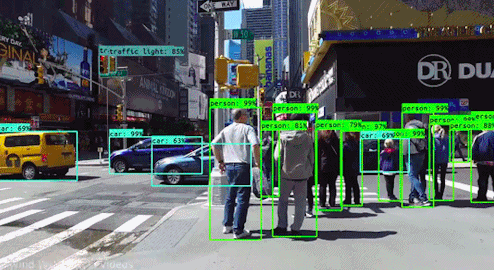
\includegraphics[width=8cm]{image.png}
\centering
\caption{Example of multiple objects in the frame making the number of computations quite large}
\end{figure}

\section{Experiment }
The authors state that experiments were conducted on Freeway, Riverraid, SpaceInvaders, BankHeist and Ms.Pacman by the Atari Games. But Space Invaders and Riverraid as well as MS Pacman and Bank Heist are similar games respectively with just changes in the objects appearance. Even with small object appearance changes the objects the F1-score changes by around 3-4\%, for which the authors have not given any explanation in the paper. Also object sensitive models work better than their corresponding Deep RL variants in different games except for the case where DQN works better than O-DQN for Space Invaders and DDQN works better than O-DDQN for Bank heist. The explanation for this was also not given the paper.It might be possible that this may be due to the number of objects being less in these games than in MS Pacman and Riverraid. Thus it may imply that this model has significant improvement when the number of objects which determine the policy of the agent are big.For example in Pacman the position of the  four ghosts and the Power Pellet determine the action to be taken. Thus it may be possible that objects are indeed quite important for making a decision about the policy.

\section{References}
1: Figure 1- https://towardsdatascience.com/google-ais-new-object-detection-competition-6dde25cf099d.\\
2: Q-Learning: Course Notes, DPOC Book, Richard Sutton and Andrew Barto,Introduction to Reinforcement Learning.\\
3:Deep Q-Learning Network:Richard Sutton and Andrew Barto,Introduction to Reinforcement Learning.\\
4: Generative Adversarial Network:Generative Adversarial Network by Ian Goodfellow.\\
5: Convolutional Neural Network: Deep Learning Book by Ian Goodfellow.\\



%%%%%%%%%%%%%%%%%%%%%%%%%%%%%%%%%%%%%%%%%%%%%%%%%%%%%%%%%%%%%%%%%%%%%%%%%%%%%%%%%%%%%%%%%%%%%%%%%%%%%%%%%%%%%%%%%%%%%%
\end{document}
